\documentclass[12pt]{article}
\usepackage[a4paper, total={6in, 8in}]{geometry}
\usepackage{amsfonts}
\usepackage{amsmath,amssymb,trimclip,adjustbox}
\usepackage{breqn}
\usepackage{geometry}
\usepackage{hyperref}
\usepackage{tabularray}
\usepackage{flafter} 
\usepackage{polski}
\usepackage[utf8]{inputenc}

\geometry{top=2cm}

\setlength{\parindent}{0pt}
\setlength{\textheight}{720pt}
\setlength{\oddsidemargin}{0pt}
\setlength{\textwidth}{480pt}

\everymath{\displaystyle}


\author{Michał Puchyr}
\title{Sprawozdanie z ćw 17 \\
WYZNACZANIE WARTOŚCI PRZYSPIESZENIA ZIEMSKIEGO}

\begin{document}
\maketitle

\section{Cel ćwiczenia}

\begin{itemize}
    \item Wyznaczenie wartości przyspieszenia ziemskiego za pomocą wahadła matematycznego.
    \item Wyznaczenie wartości przyspieszenia ziemskiego za pomocą wahadła fizycznego.
\end{itemize}

\section{Opis ćwiczenia - wstęp teoretyczny}

Pomiary, które zostały wykonane miały na celu wyznaczenie \textbf{przyśpieszenia ziemskiego} w miejscu
gdzie był wykonywany eksperyment (Wrocław - $51^{\circ}06'27.7" N, 17^{\circ}03'40.6" E$). \\

\textbf{Przyspieszenie ziemskie} -- przyspieszenie grawitacyjne ciał swobodnie spadających na Ziemię, bez oporów ruchu.

Wartość przyspieszenia ziemskiego zależy od szerokości geograficznej oraz wysokości nad poziomem morza. 
Wraz z wysokością przyspieszenie maleje odwrotnie proporcjonalnie do kwadratu odległości do środka Ziemi 
i jest wynikiem zmniejszania się siły grawitacji zgodnie z prawem powszechnego ciążenia. 

Zmniejszanie się przyspieszenia ziemskiego wraz ze zmniejszaniem szerokości geograficznej 
jest spowodowane działaniem pozornej siły odśrodkowej, która powstaje na skutek ruchu obrotowego Ziemi. 

Ponieważ siła ta jest proporcjonalna do odległości od osi obrotu, stąd największą wartość osiąga na równiku. 
Ponieważ siła odśrodkowa ma tu zwrot przeciwny do siły grawitacji, 
przyspieszenie ziemskie na równiku osiąga najmniejszą wartość. 

Dodatkowe zmniejszenie przyspieszenia ziemskiego w okolicach równika spowodowane jest spłaszczeniem Ziemi 
(większą odległością od środka Ziemi).

Do obliczeń niewymagających wysokiej precyzji przyjmuje się tzw. przyśpieszenie ziemskie normalne tj.:
$$ g_n = 9,80665 \frac{m}{s^2} $$

Przyśpieszenie ziemskie we Wrocławiu wynosi około :
$$ g = 9,8115 \frac{m}{s^2} $$

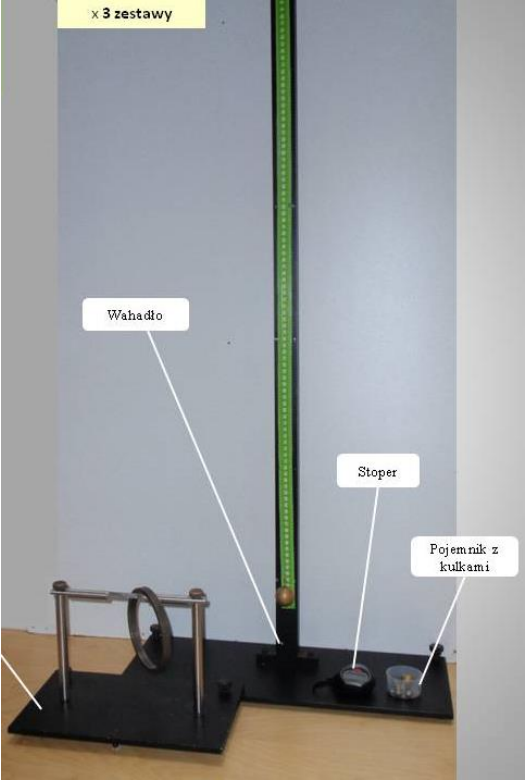
\includegraphics[scale=0.6]{schemat.png}

Stanowisko pomiarowe \\

Wykaz przyrządów : 
\begin{itemize}
    \item Wahadło matematyczne
    \item Metalowy pierścień
    \item Waga laboratoryjna
    \item Suwmiarka
    \item Stoper
    \item Przymiar
\end{itemize}

\section{Pomiary układów}

\begin{table}[!htbp]
    \centering
    \begin{adjustbox}{width=0.4\textwidth}
    \begin{tabular}{|c|c|}
    \hline
    \multicolumn{2}{|c|}{Przyjęte niepewności} \\
    \hline
    Niepewność & Wartość \\ \hline
    u(t)[s] & 0,0058 \\ \hline
    u(n) & 1 \\ \hline
    \end{tabular}
\end{adjustbox}
\end{table}

\begin{table}[!htbp]
    \centering
    \begin{adjustbox}{width=1\textwidth}
    \begin{tabular}{|c|c|c|c|c|c|c|c|c|c|c|}
    \hline
    \multicolumn{11}{|c|}{Wyniki pomiarów i obliczenia dla wahadła matematycznego} \\
    \hline
    lp. & l$_i$[m] & t$_i$[s] & l$_{sr}$[m] & $\overline{t}$[s] & T$\left[ \frac{1}{s} \right]$ & u(T)$\left[\frac{1}{s}\right]$ & T$_{sr}\left[ \frac{1}{s} \right]$ & g$\left[ \frac{m}{s^2} \right]$ & $\overline{g} \left[ \frac{m}{s^2} \right]$ & u(g)$\left[ \frac{m}{s^2} \right] $ 
    \\[10pt] \hline
    1 & 0,390 & 125,15 & 0,391 & 125,01 & 1,26 & 0,013 & 1,25 & 9,699 & 9,808 & 0,25\\
    2 & 0,390 & 124,87 & ~ & ~ & 1,25          & 0,013 & ~     & 9,854 & ~ & 0,26\\
    3 & 0,391 & 124,99 & ~ & ~ & 1,25          & 0,013 & ~     & 9,880 & ~ & 0,26\\ \hline
    4 & 0,500 & 141,33 & 0,500 & 141,44 & 1,42 & 0,015 & 1,42  & 9,790 & ~ & 0,24\\
    5 & 0,501 & 141,46 & ~ & ~ & 1,42          & 0,015 & ~     & 9,809 & ~ & 0,24\\
    6 & 0,499 & 141,51 & ~ & ~ & 1,42          & 0,015 & ~     & 9,770 & ~ & 0,24\\ \hline
    7 & 0,613 & 156,48 & 0,614 & 156,47 & 1,57 & 0,016 & 1,57  & 9,818 & ~ & 0,23\\
    8 & 0,613 & 156,78 & ~ & ~ & 1,57          & 0,016 & ~     & 9,818 & ~ & 0,23\\
    9 & 0,614 & 156,13 & ~ & ~ & 1,57          & 0,016 & ~     & 9,834 & ~ & 0,23\\ \hline
    \end{tabular}
\end{adjustbox}
\end{table}

\section{Przykładowe obliczenia}

\subsection{Obliczenia dla pomiarów wahadła matematycznego}

Obliczenie niepewności pomiaru długości wahadła :
$$ u(l) = \frac{0,01}{\sqrt{3}} = 0,00578 \approx 0,0058[m] $$

Obliczenie okresu wahnięć pomiaru :
$$ T = \frac{t_i}{n} = \frac{125,15}{100} = 1,2515 \approx 1,26[s] $$

Obliczenie niepewności pomiaru okresu : 
$$ u(T) = \sqrt{ \left( \frac{\partial T}{\partial t} \right)^2 \cdot u^2(t) + \left( \frac{\partial T}{\partial n} \right)^2 \cdot u^2(n) }
= \sqrt{ \left( \frac{1}{n^2} \right)^2 \cdot u^2(t) + \left( \frac{-t}{n^2} \right)^2 \cdot u^2(n) } $$
$$ = \sqrt{ \left( \frac{1}{100^2} \right)^2 \cdot 0,0058^2 + \left( \frac{-125,15}{100^2} \right)^2 \cdot 1^2 } = 0,01251 \approx 0,013 \left[ \frac{1}{s} \right]$$

Obliczenie przyśpieszenia ziemskiego : 
$$ g = 4\pi^2 \frac{l}{T^2} = 4\pi^2 \frac{0,390}{1,26^2} = 9,69802 \approx 9,699 \left[ \frac{m}{s^2} \right] $$

Obliczenie niepewności pomiaru przyśpieszenia ziemskiego :
$$ u(g) = \sqrt{ \left( \frac{\partial g}{\partial l} \right)^2 \cdot u^2(l) + \left( \frac{\partial g}{\partial T} \right)^2 \cdot u^2(T) }
= \sqrt{ \left( \frac{4 \pi^2}{T^2} \right)^2 \cdot u^2(l) + \left( \frac{-8 \pi^2 l}{T^3} \right)^3 \cdot u^2(T) } $$
$$ = \sqrt{ \left( \frac{4\pi^2}{1,26^2} \right)^2 \cdot 0,0058^2 + \left( \frac{-8\pi^2 \cdot 0,39}{1,26^3} \right)^2 \cdot 0,013^2 }
= 0,24667 \approx 0,25 \left[ \frac{m}{s^2} \right] $$

Obliczenie średniej długości wahadła :
$$ l_{sr} = \frac{\sum\limits_{i=1}^{n} l_i}{n} = \frac{1,171}{3} = 0,39033 \approx 0,391[m]$$

Obliczenie średniej czasu pomiarów : 
$$ \overline{t} = \frac{\sum\limits_{i=1}^{n} t_i}{n} = \frac{375,01}{3} = 125,0033 \approx 125,01[s] $$

Obliczenie średniej długości okresu pomiarów :
$$ T_{sr} = \frac{\sum\limits_{i = 1}^{n} T_i}{n} = \frac{3,76}{3} = 1,25333 \approx 1,25[s] $$

\subsection{Obliczenia dla pomiarów wahadła fizycznego}

Obliczenie momentu bezwładności :
$$ I = I_0 + m \frac{d^2}{4} $$

\end{document}